\section{Цель работы}
Для заданного объекта управления синтезировать оптимальный наблюдатель (фильтр Калмана).



\section{Теоретические сведения}
Рассматриваемый объект управления:
\begin{equation}
    \begin{aligned}
        & \dot{x} = A x + b u + G w, \quad x(0), \\
        & y = C x + v
    \end{aligned}
\end{equation}
где $w$, $v$~--- сигналы вида <<белый шум>> с нулевыми математическими ожиданиями и автокорреляционными функциями 
\begin{equation}
    M \{ w(t) w^T(\tau) \} = W \delta(t - \tau),
    \qquad
    M \{ v(t) v^T(\tau) \} = V \delta(t - \tau),
\end{equation}
где $M\{\cdot\}$~--- математическое ожидание, c известными постоянными спектральными плотностями (энергиями) $W$ и $V$ соответственно.

Структура синтезируемого наблюдателя
\begin{equation}
    \dot{\hat{x}} = A \hat{x} + b u + L (y - C \hat{x}), \quad \hat{x}(0),
\end{equation}
где оптимальное значение матрицы $L$, обозначенное как $L_\text{опт}$, рассчитывается на основе уравнения Риккати:
\begin{align}
    & A^T P + P A + G W G^T - P C^T V^{-1} C P = 0, \label{eq_riccati_equation}\\
    & L_\text{опт} = P C^T V^{-1} \label{eq_L_equation} \ldotp
\end{align}
Данный наблюдатель при $L = L_\text{опт}$ генерирует оценку $\hat{x}$ такую, что
\begin{equation}
    \| x(t) - \hat{x}(t) \| \leqslant \Delta, \quad \forall t \geqslant T,
\end{equation}
где $\Delta$ и $T$~--- максимальная ошибка и время настройки наблюдателя соответственно, и минимизирует следующий функционал
\begin{equation}\label{eq_perfomance_index}
    J = M \{ e^T_\text{н} e_\text{н} \},
\end{equation}
где $e_\text{н} = x - \hat{x}$~--- ошибка наблюдения.


\section{Исходные данные}
Варианту \textnumero2 соответствует следующий набор исходных данных:
\begin{equation}
    A =
    \begin{bmatrix}
        0 &  1 \\
        1 & -1
    \end{bmatrix}\!\!,
    \quad
    b =
    \begin{bmatrix}
        2 \\ 1
    \end{bmatrix}\!\!,
    \quad
    C =
    \begin{bmatrix}
        1 & 0
    \end{bmatrix}
    \quad
    G = I,
    \quad
    W =
    \begin{bmatrix}
        2 & 1.5 \\
        1.5 & 2
    \end{bmatrix}\!\!,
    \quad
    V = 2 \ldotp
\end{equation}



\section{Результаты практических действий}
Эквивалентная форма расчетного выражения для критерия качества:
\begin{equation}
    J(t) = M \{ e^T_\text{н} e_\text{н} \} = \frac{1}{t - t_0} \int\limits_{t_0}^{t} e^T_\text{н}(\tau) e_\text{н}(\tau)\, d\tau \ldotp
\end{equation}

Для получения вектора случайных величин~$w_0$ с желаемой матрицей ковариации~$W$ из вектора случайных величин~$w^*$, чья матрица ковариации равна единичной матрице соответствующих размеров, может быть использовано следующее выражение:
\begin{equation}
    w_0 = R^T w^*\!\!,
\end{equation}
где $R$ получается из разложения Холецкого матрицы~$W$:
\begin{equation}
    W = R^T R \ldotp
\end{equation}


Результаты решения уравнений~\eqref{eq_riccati_equation} и~\eqref{eq_L_equation}:
\begin{equation}
    P = \begin{bmatrix}3.7419999&2.5006408\cr 2.5006408&1.9373397\cr \end{bmatrix}\!\!,
    \qquad
    L_\text{опт} = \begin{bmatrix}1.8709999\cr 1.2503204\cr\end{bmatrix}\!\!\ldotp
\end{equation}

Графики переходных процессов в рассматриваемой системе при различных значениях матриц $L$, $W$ и $V$ показаны на рисунках~\ref{img_graphs_2}--\ref{img_graphs_52},
а использованная для их получения схема моделирования~--- на рисунке~\ref{img_modeling_scheme}.

\begin{figure}[h!]
    \centering
    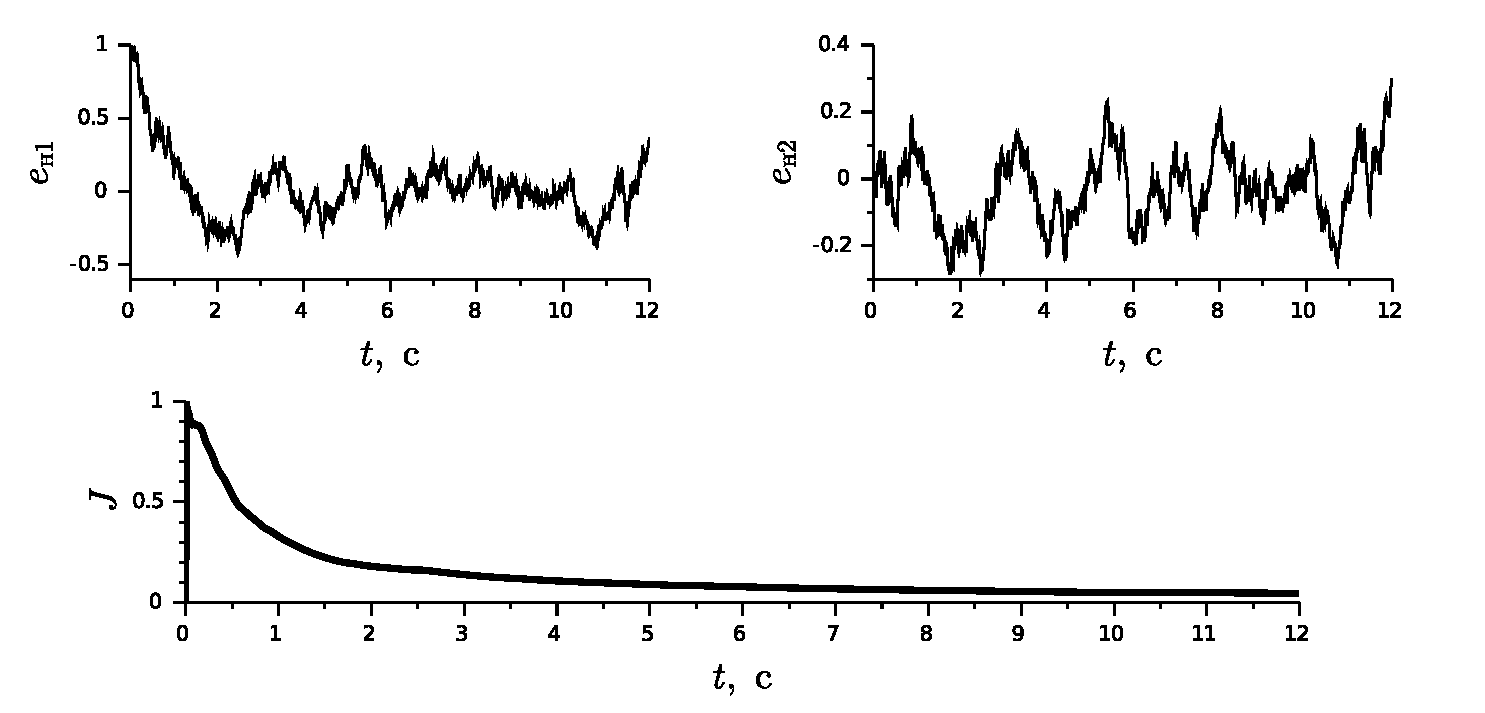
\includegraphics[width=1.0\textwidth]{graphs_2.pdf}
    \vspace{0cm}
    \caption{Графики переходных процессов при номинальных $W$ и $V$ и $L = L_\text{опт}$.}
    \label{img_graphs_2}
\end{figure}

\begin{figure}[h!]
    \centering
    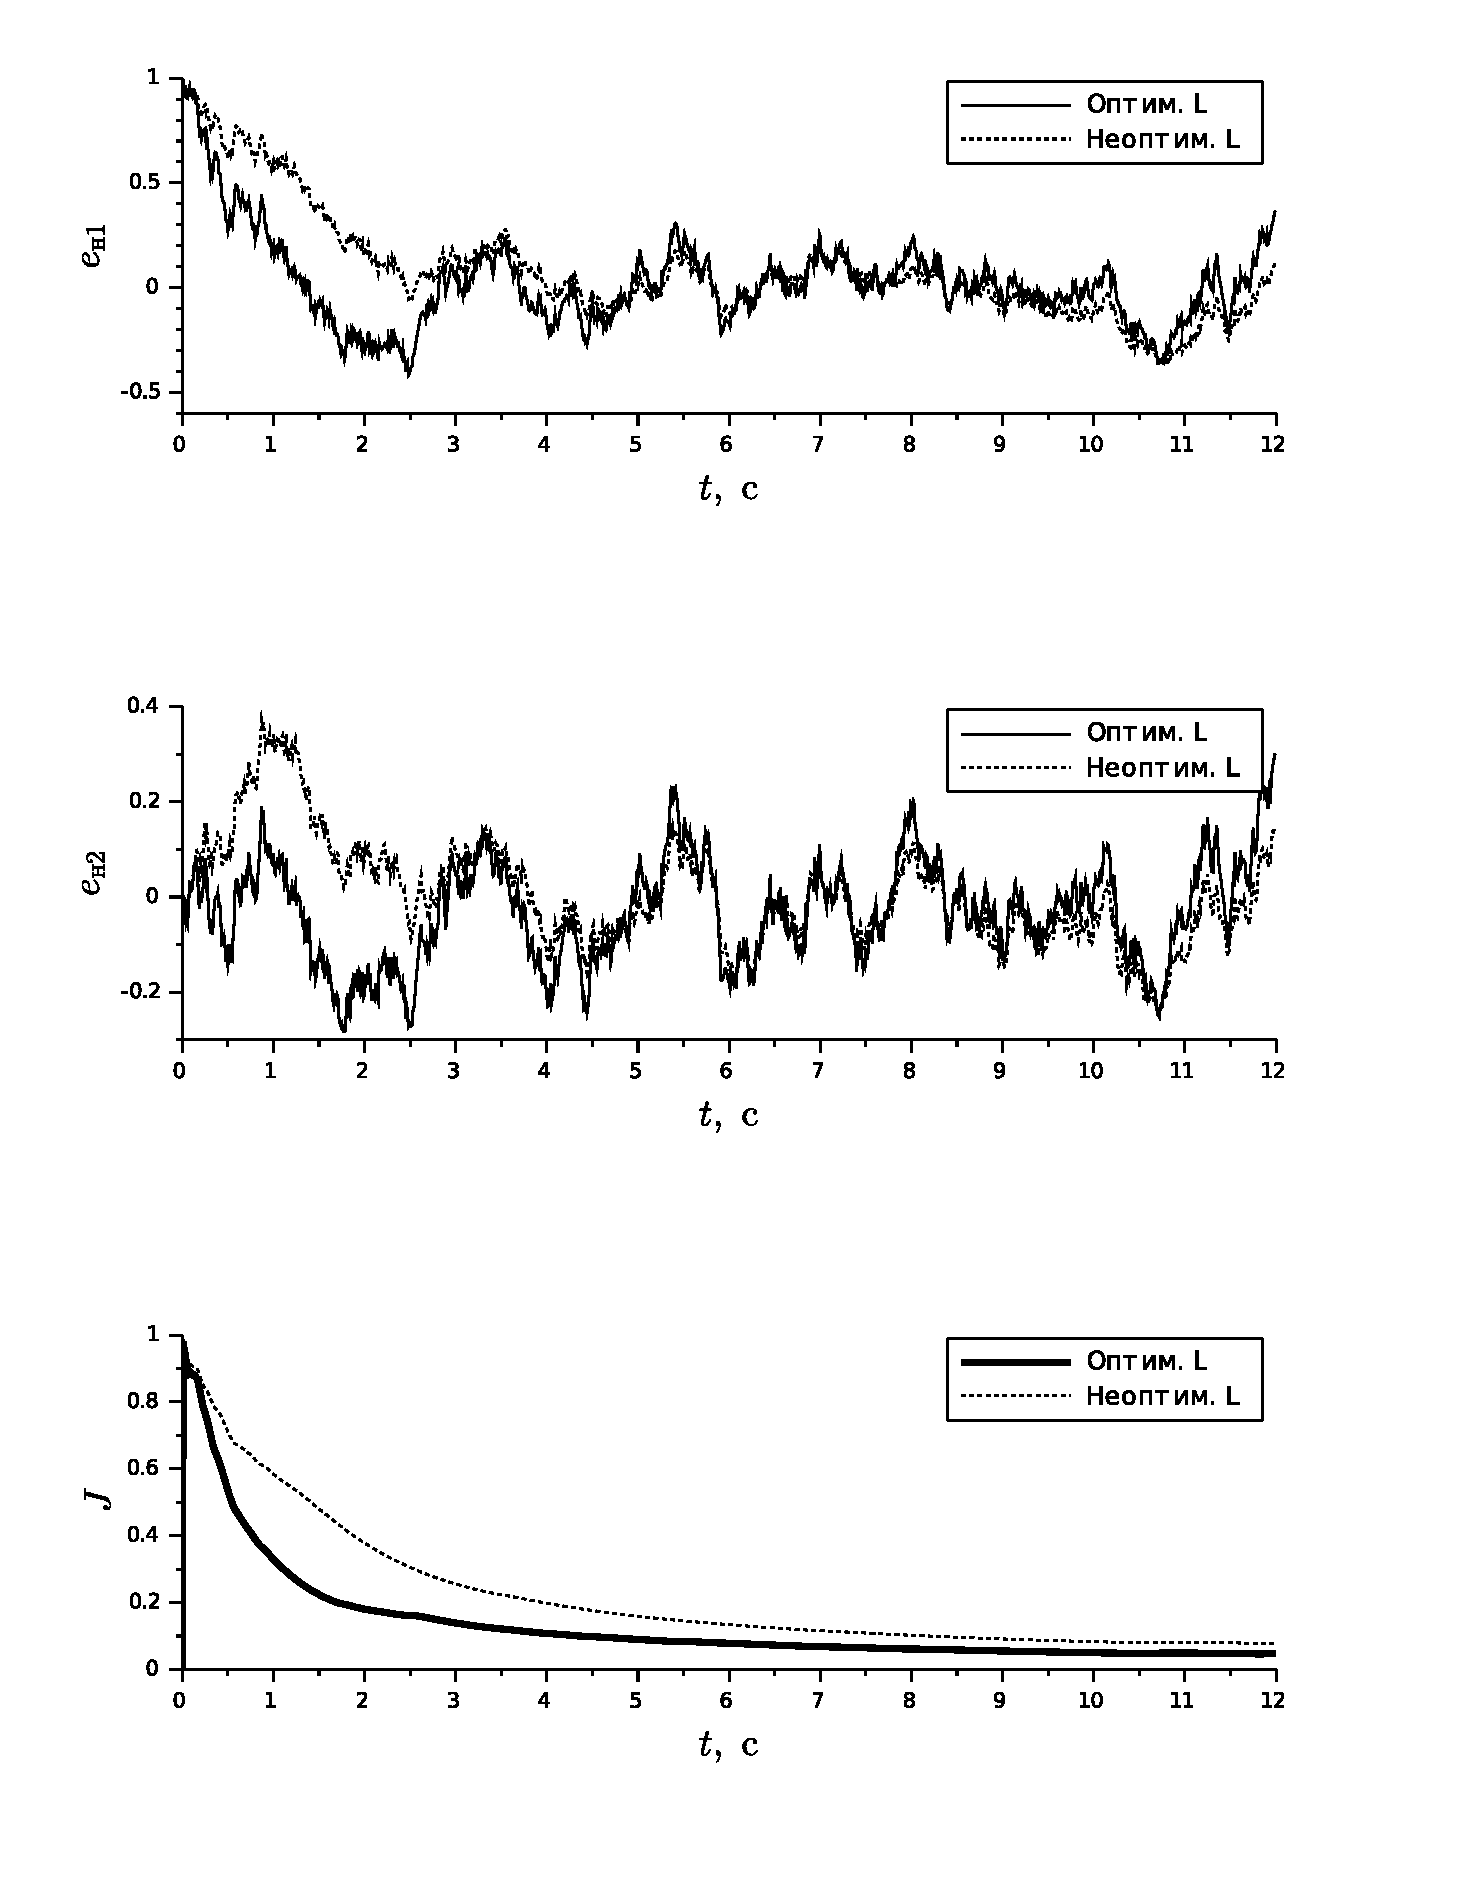
\includegraphics[width=1.0\textwidth]{graphs_31.pdf}
    \vspace{0cm}
    \caption{Графики переходных процессов при номинальных $W$ и $V$ и $L = 0.5 L_\text{опт}$ в сравнении с графиками с рисунка~\ref{img_graphs_2}.}
    \label{img_graphs_31}
\end{figure}

\begin{figure}[h!]
    \centering
    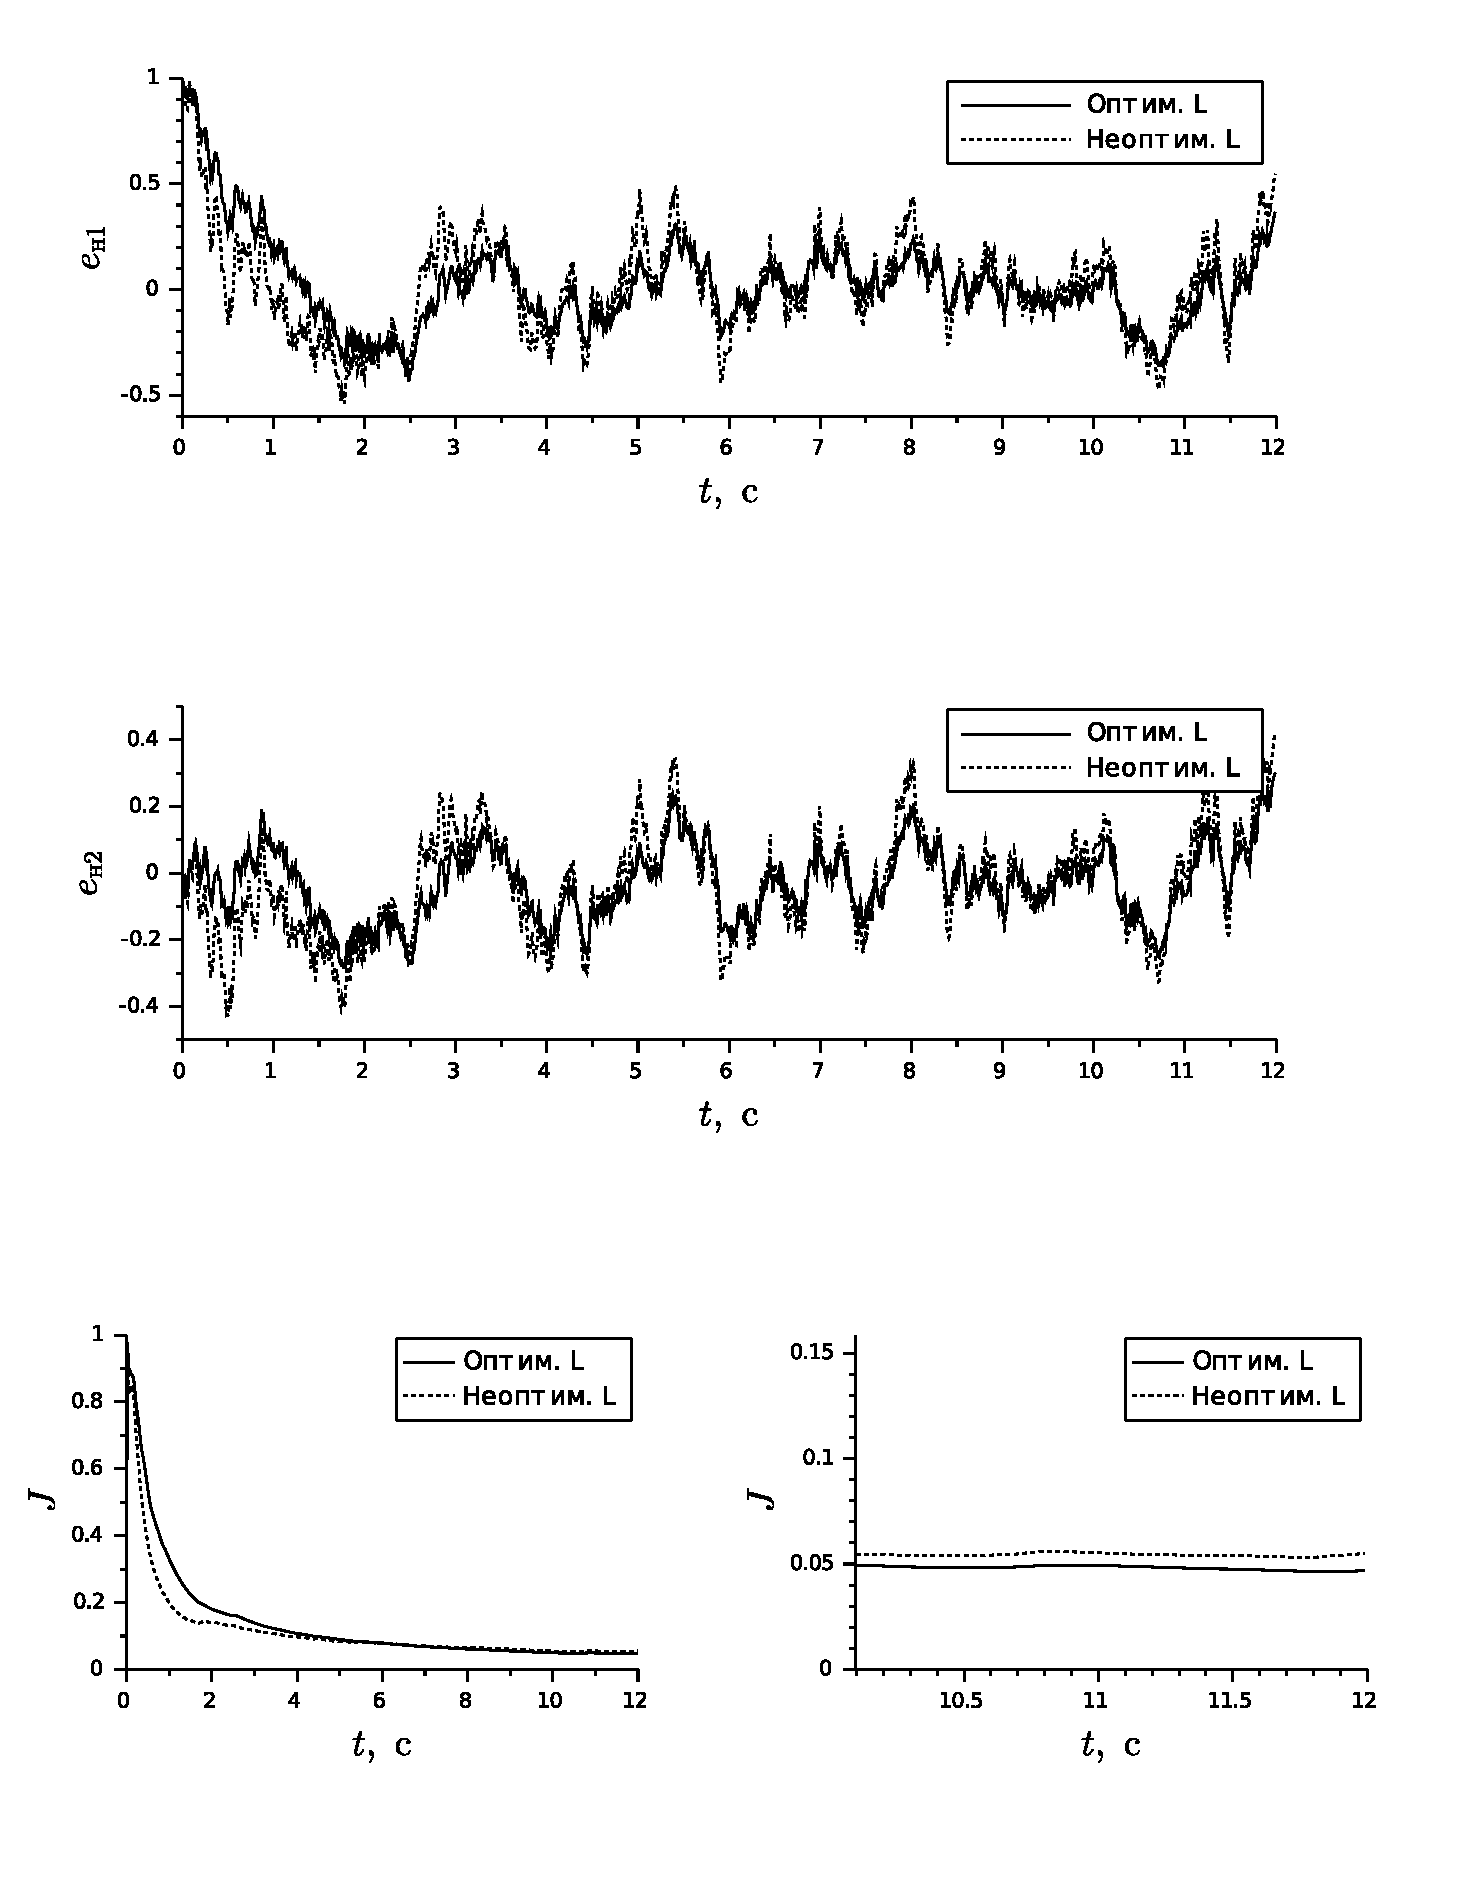
\includegraphics[width=1.0\textwidth]{graphs_32.pdf}
    \vspace{0cm}
    \caption{Графики переходных процессов при номинальных $W$ и $V$ и $L = 2 L_\text{опт}$ в сравнении с графиками с рисунка~\ref{img_graphs_2}.}
    \label{img_graphs_32}
\end{figure}

\begin{figure}[h!]
    \centering
    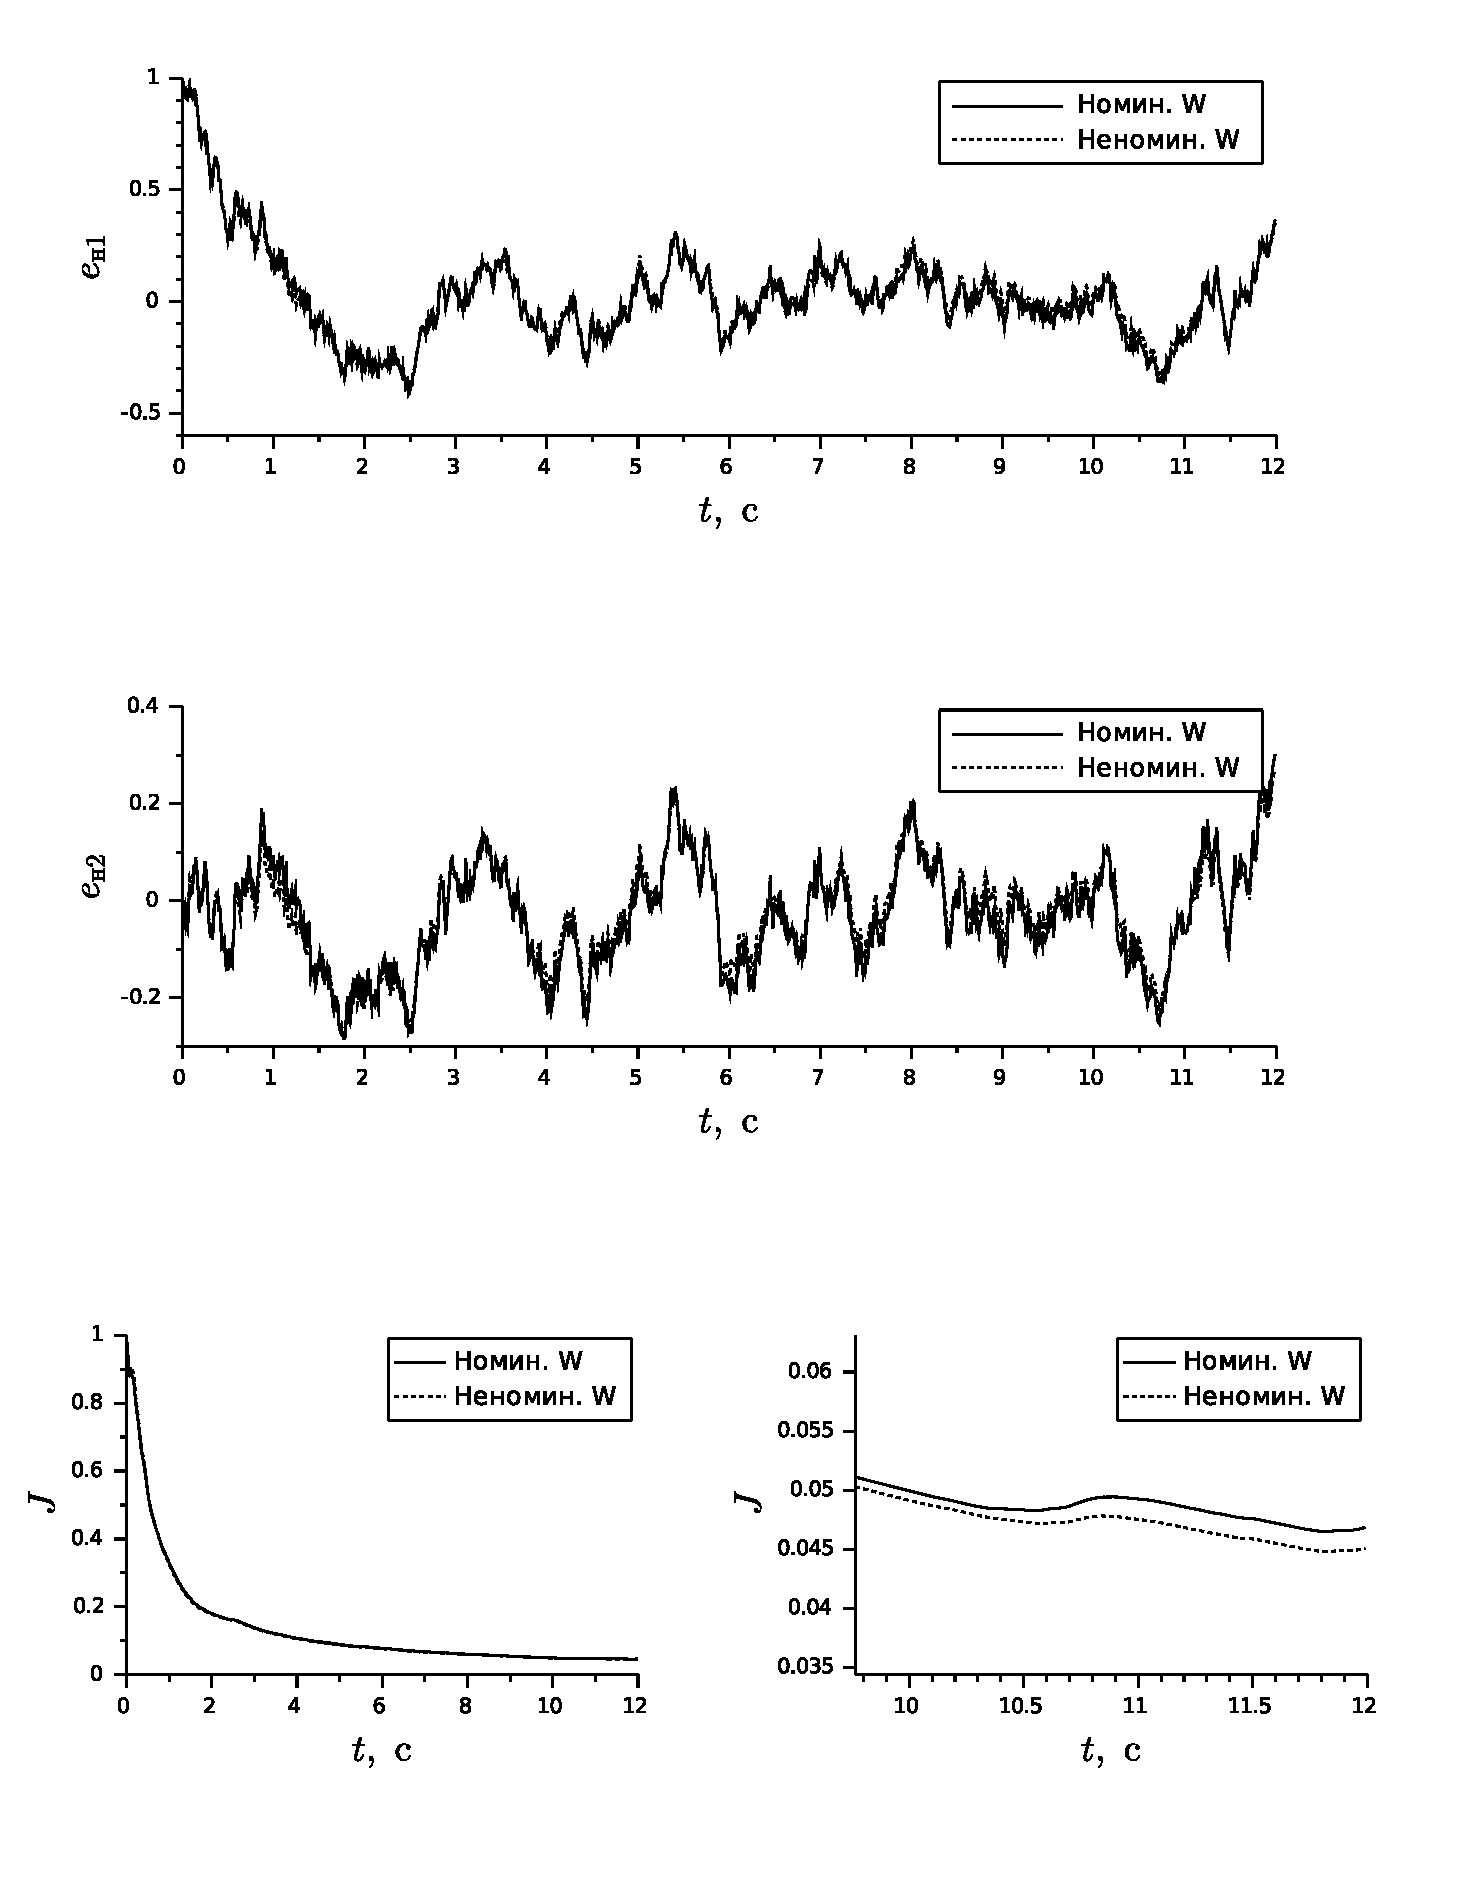
\includegraphics[width=1.0\textwidth]{graphs_41.pdf}
    \vspace{0cm}
    \caption{Графики переходных процессов при номинальной $V$, оптимальной~$L$ и вдвое уменьшенной~$W$ в сравнении с графиками с рисунка~\ref{img_graphs_2}.}
    \label{img_graphs_41}
\end{figure}

\begin{figure}[h!]
    \centering
    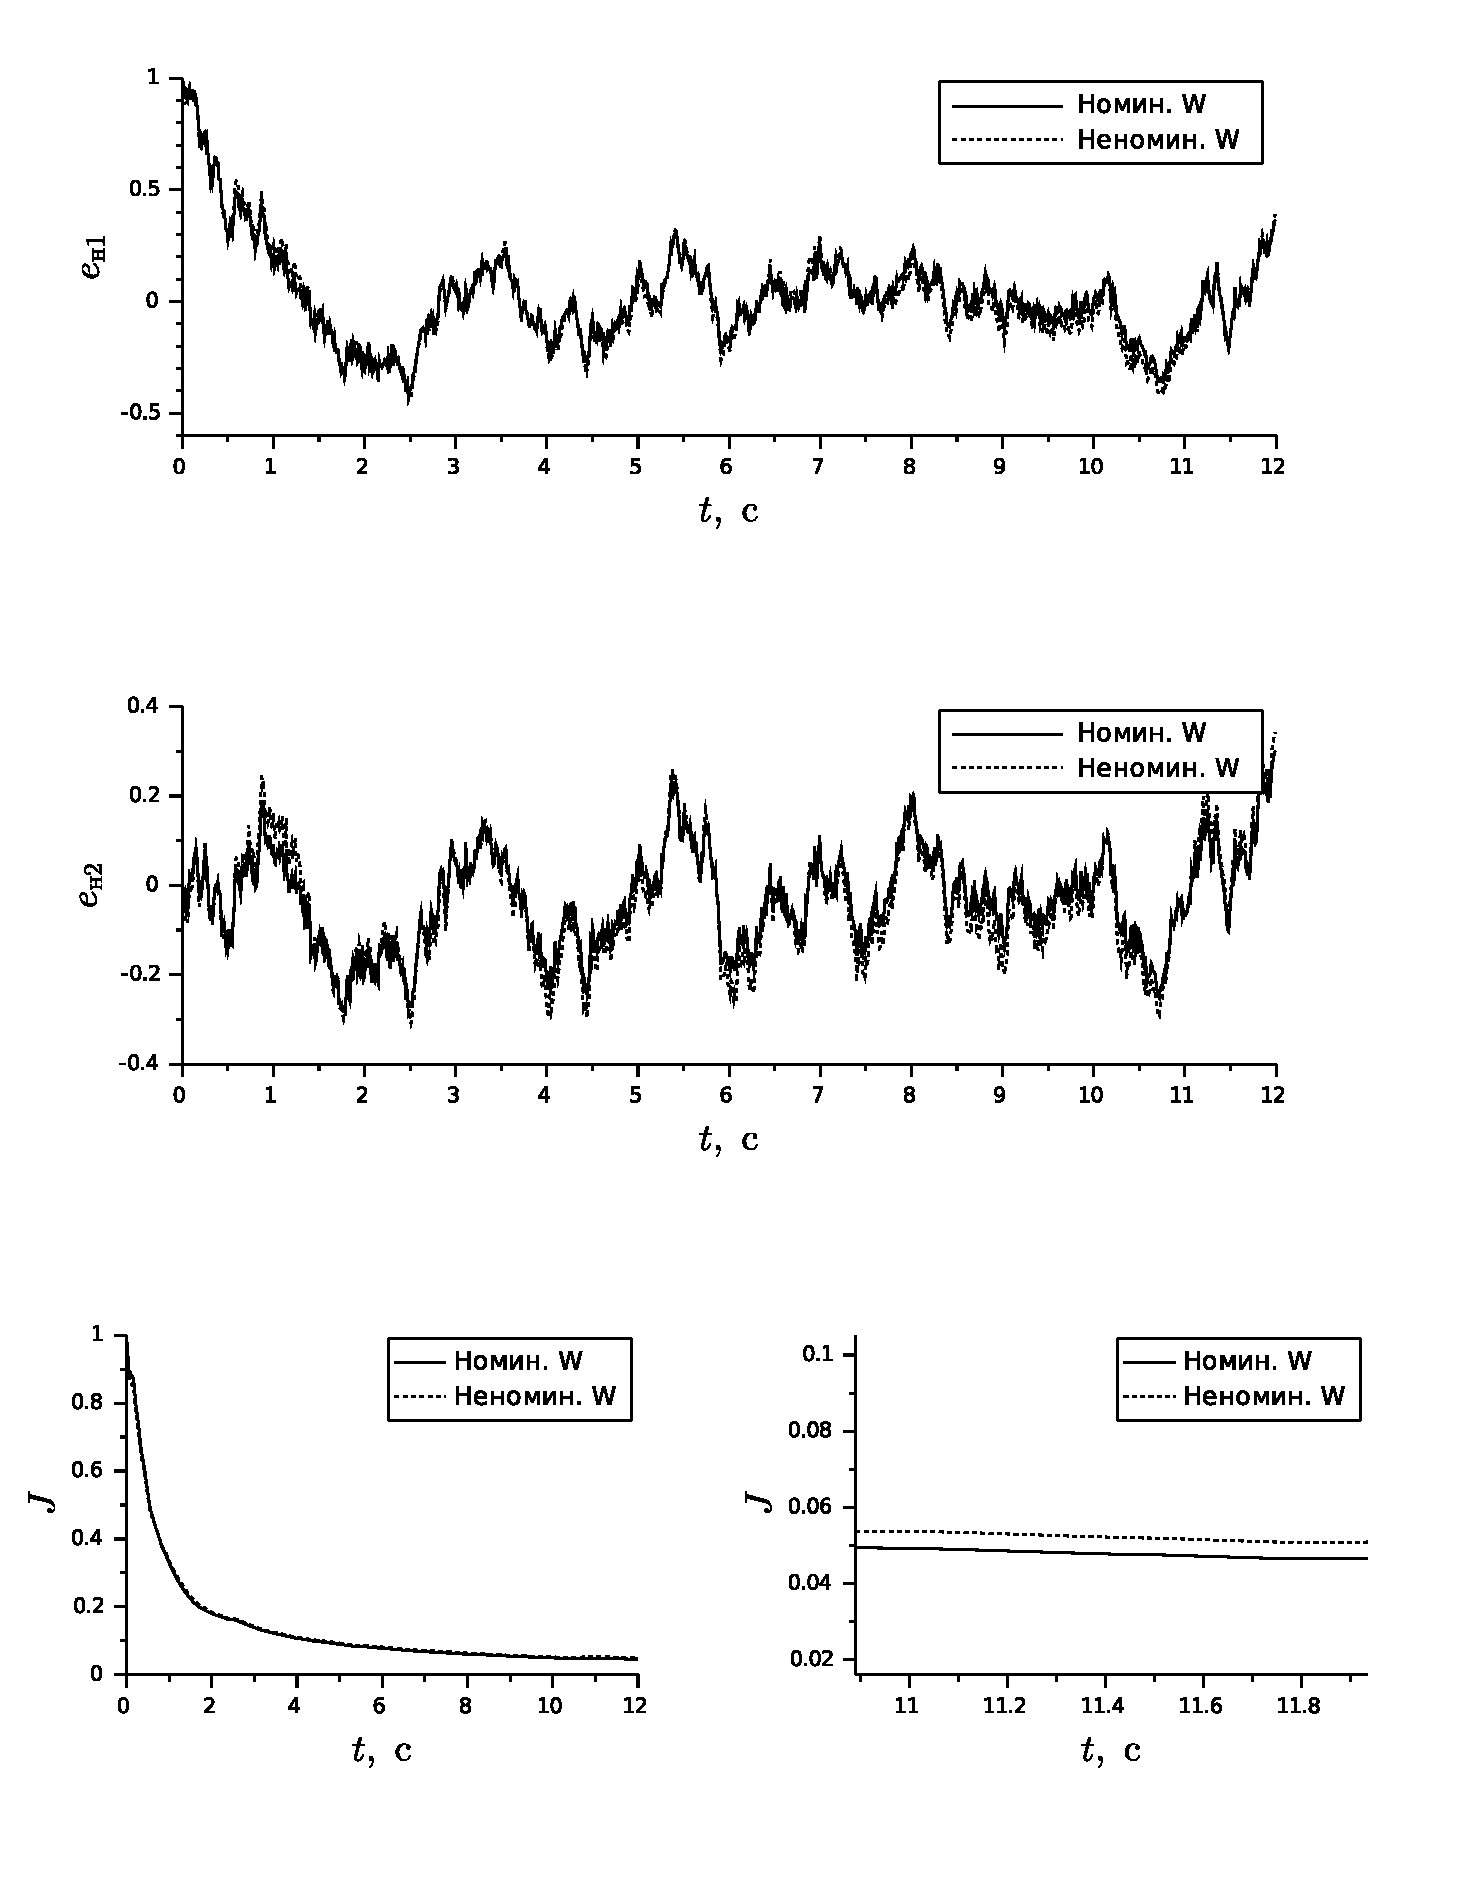
\includegraphics[width=1.0\textwidth]{graphs_42.pdf}
    \vspace{0cm}
    \caption{Графики переходных процессов при номинальной $V$, оптимальной~$L$ и удвоенной~$W$ в сравнении с графиками с рисунка~\ref{img_graphs_2}.}
    \label{img_graphs_42}
\end{figure}

\begin{figure}[h!]
    \centering
    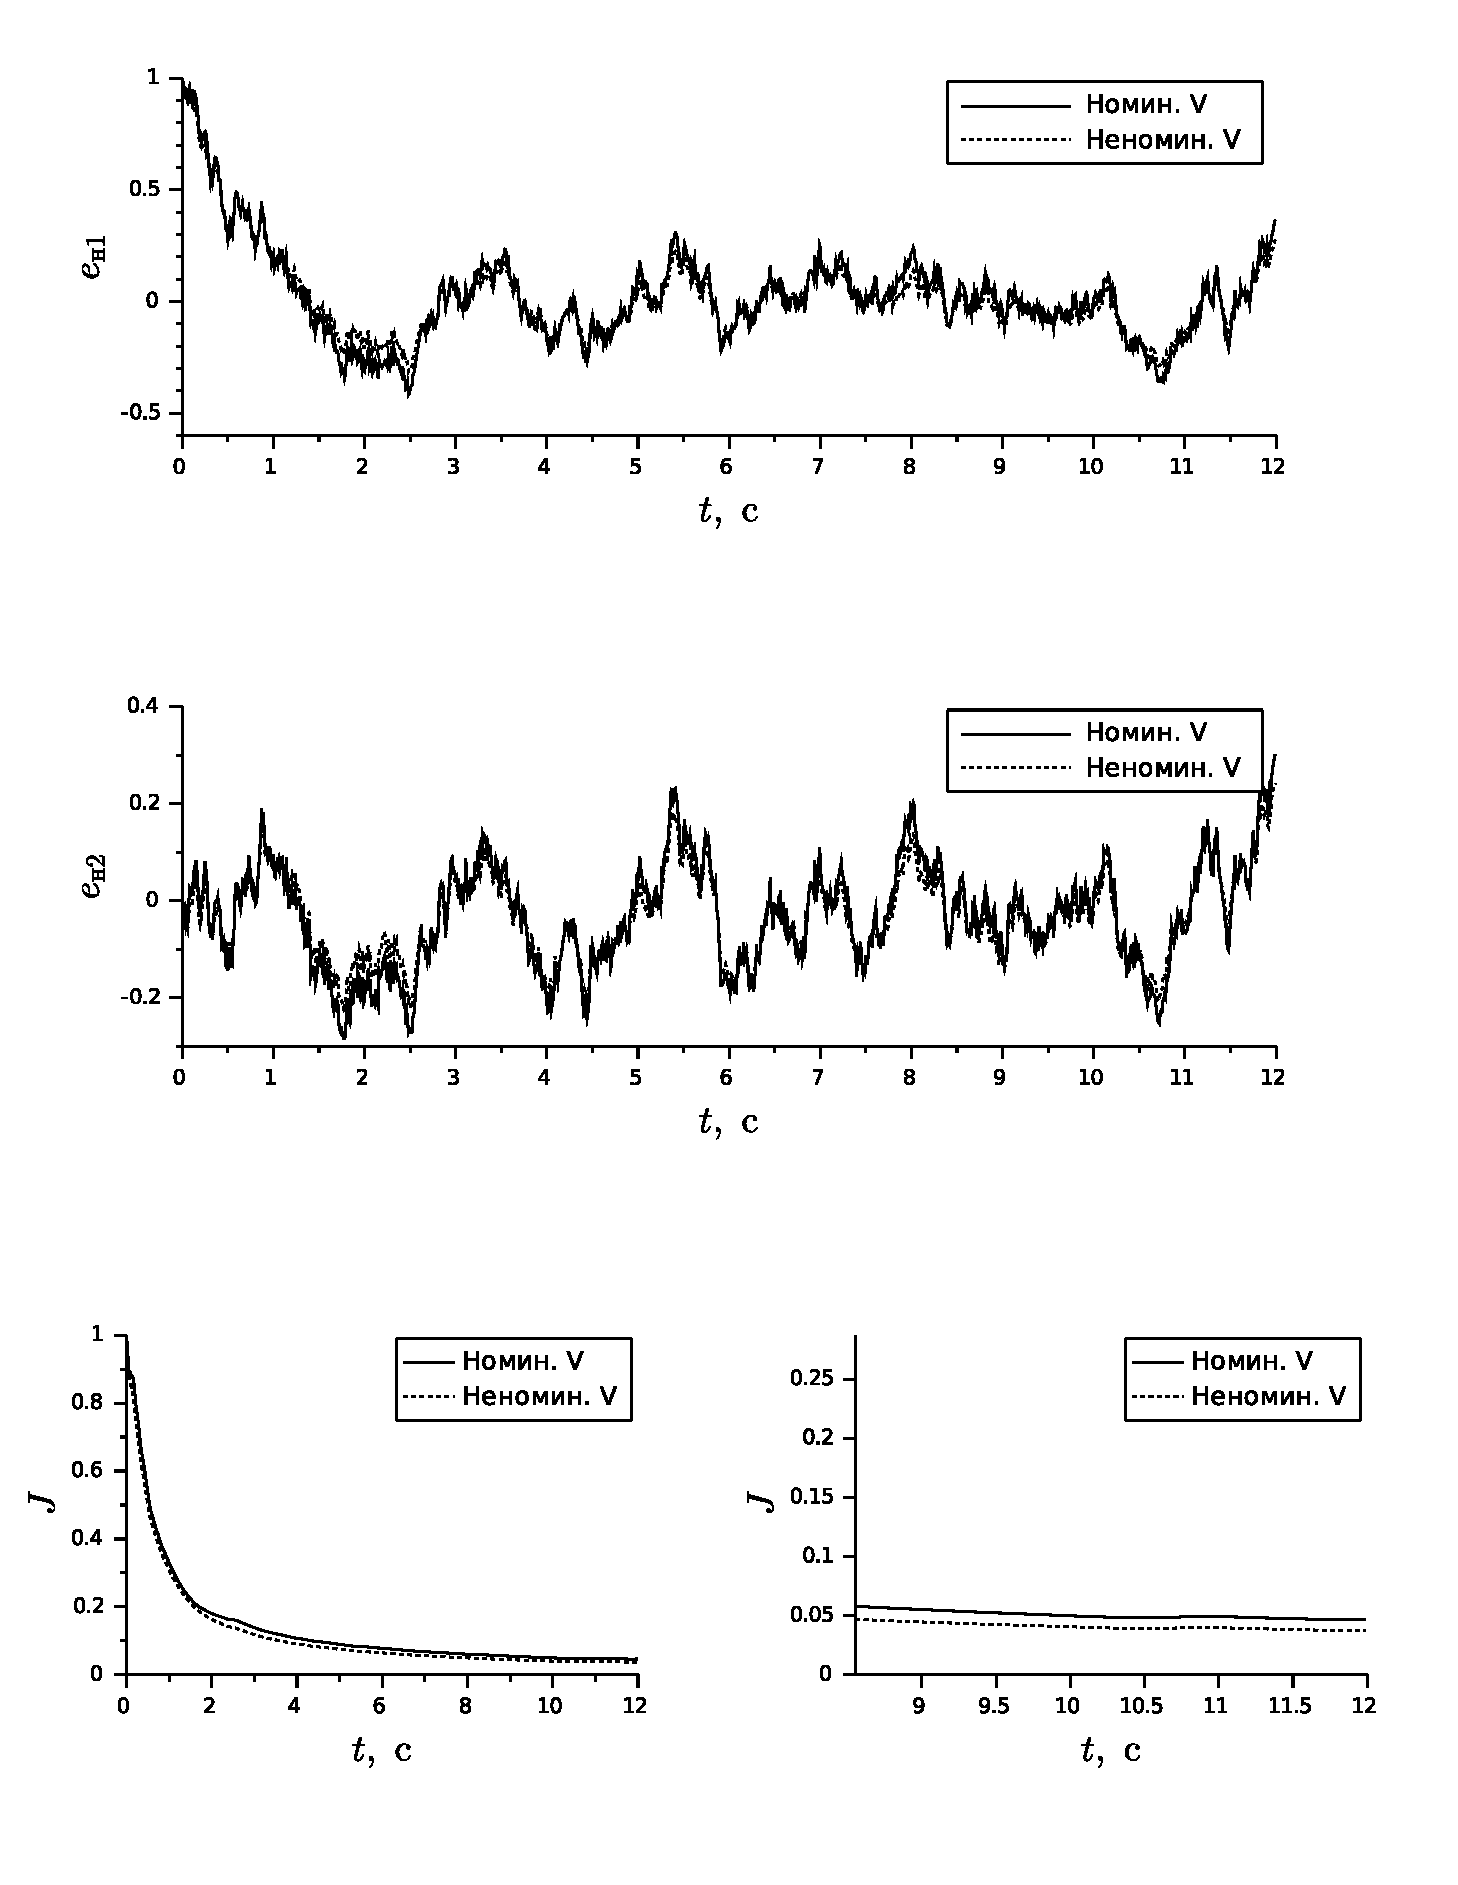
\includegraphics[width=1.0\textwidth]{graphs_51.pdf}
    \vspace{0cm}
    \caption{Графики переходных процессов при номинальной $W$, оптимальной~$L$ и вдвое уменьшенной~$V$ в сравнении с графиками с рисунка~\ref{img_graphs_2}.}
    \label{img_graphs_51}
\end{figure}

\begin{figure}[h!]
    \centering
    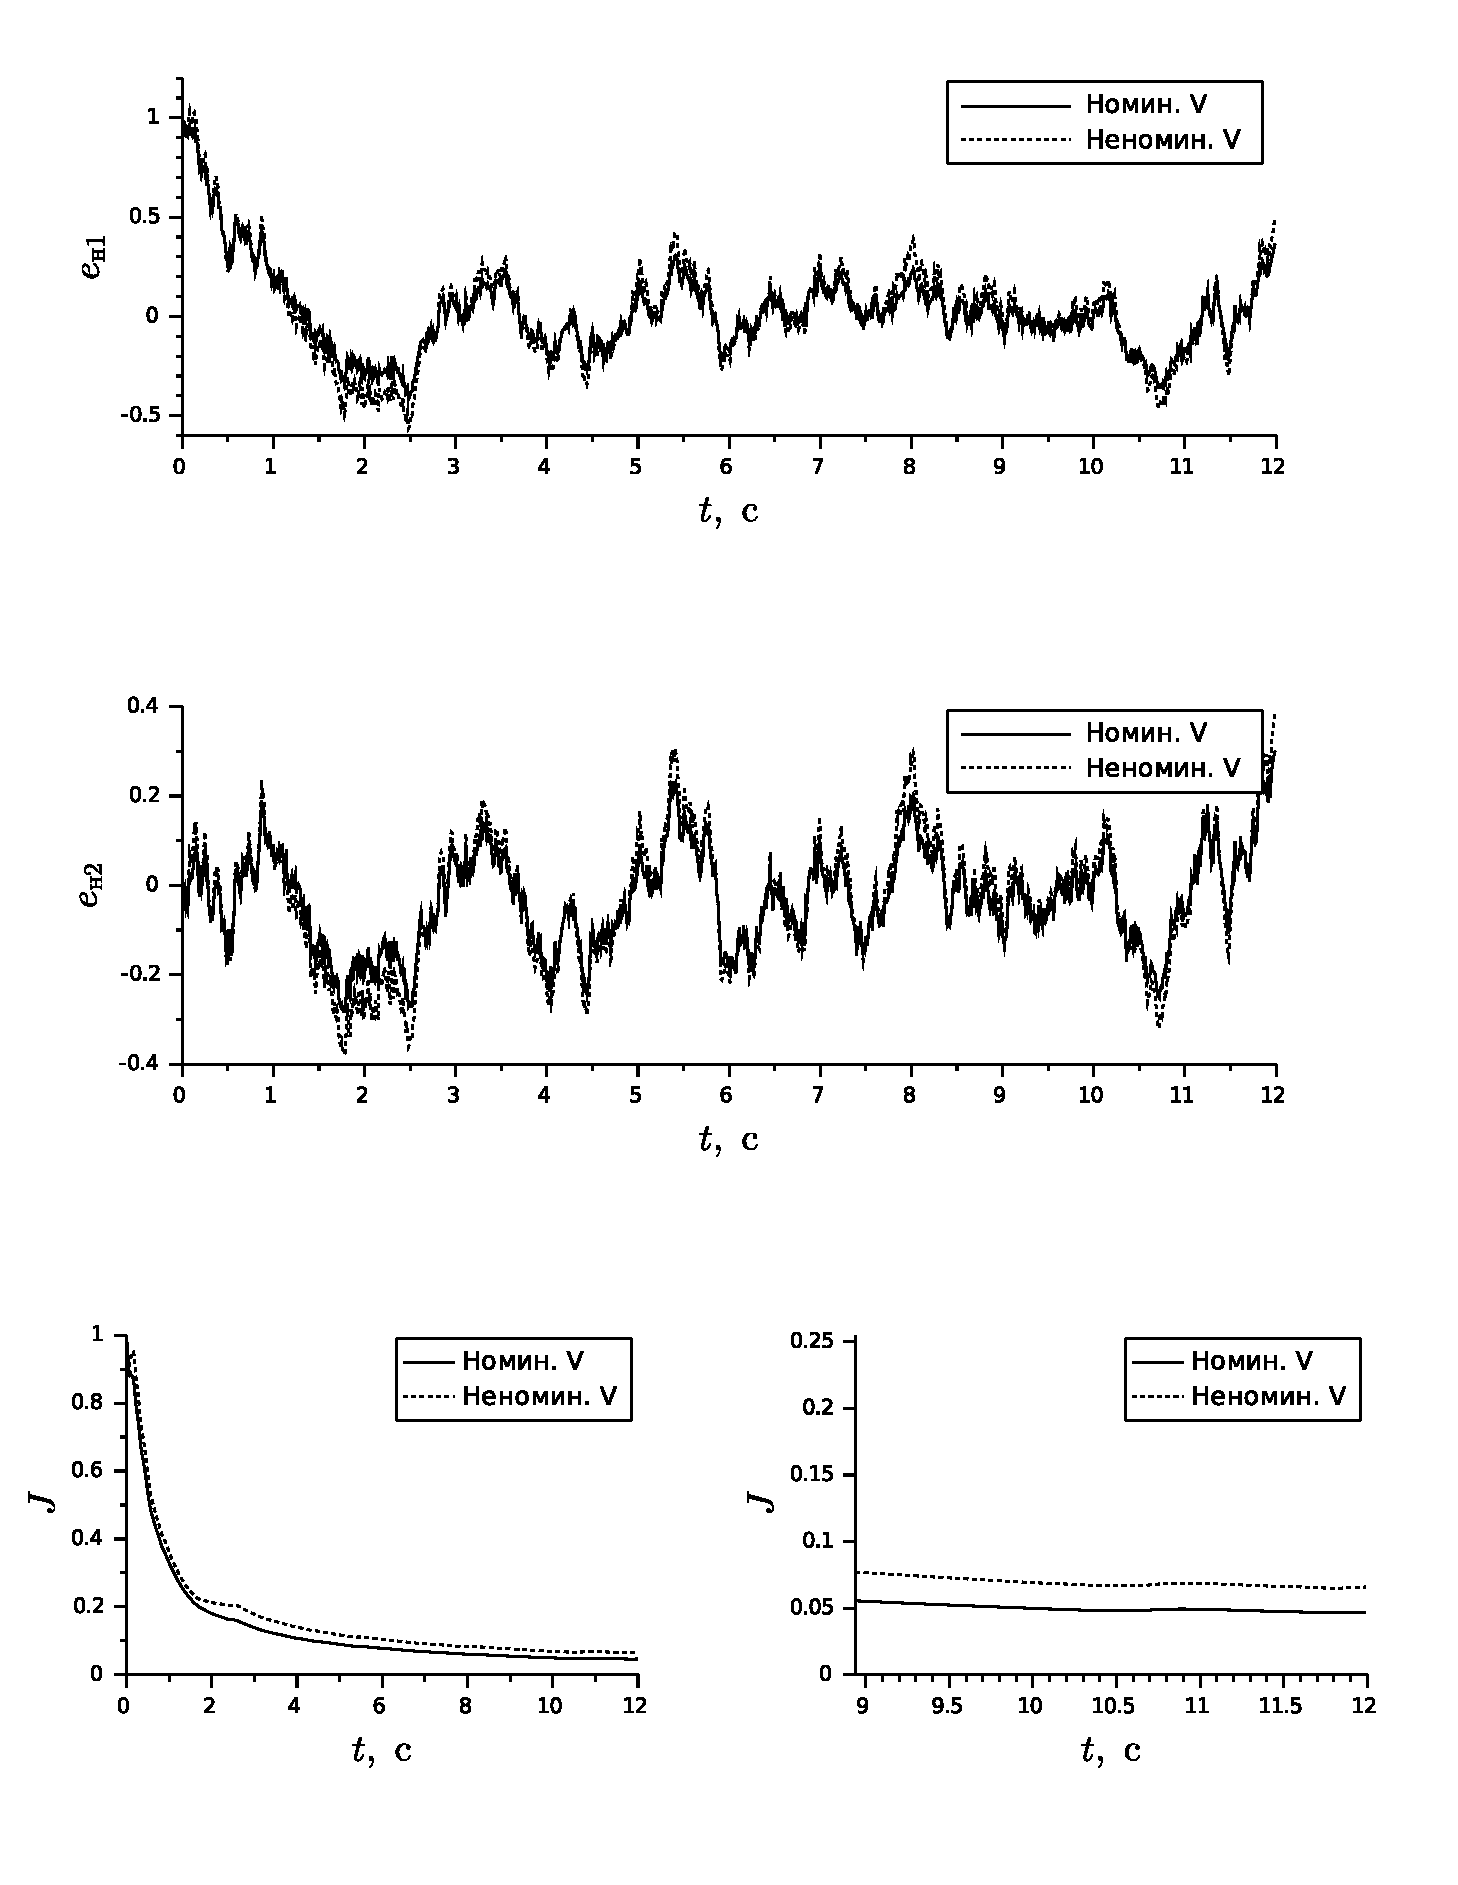
\includegraphics[width=1.0\textwidth]{graphs_52.pdf}
    \vspace{0cm}
    \caption{Графики переходных процессов при номинальной $W$, оптимальной~$L$ и удвоенной~$V$ в сравнении с графиками с рисунка~\ref{img_graphs_2}.}
    \label{img_graphs_52}
\end{figure}

\begin{figure}[h!]
    \centering
    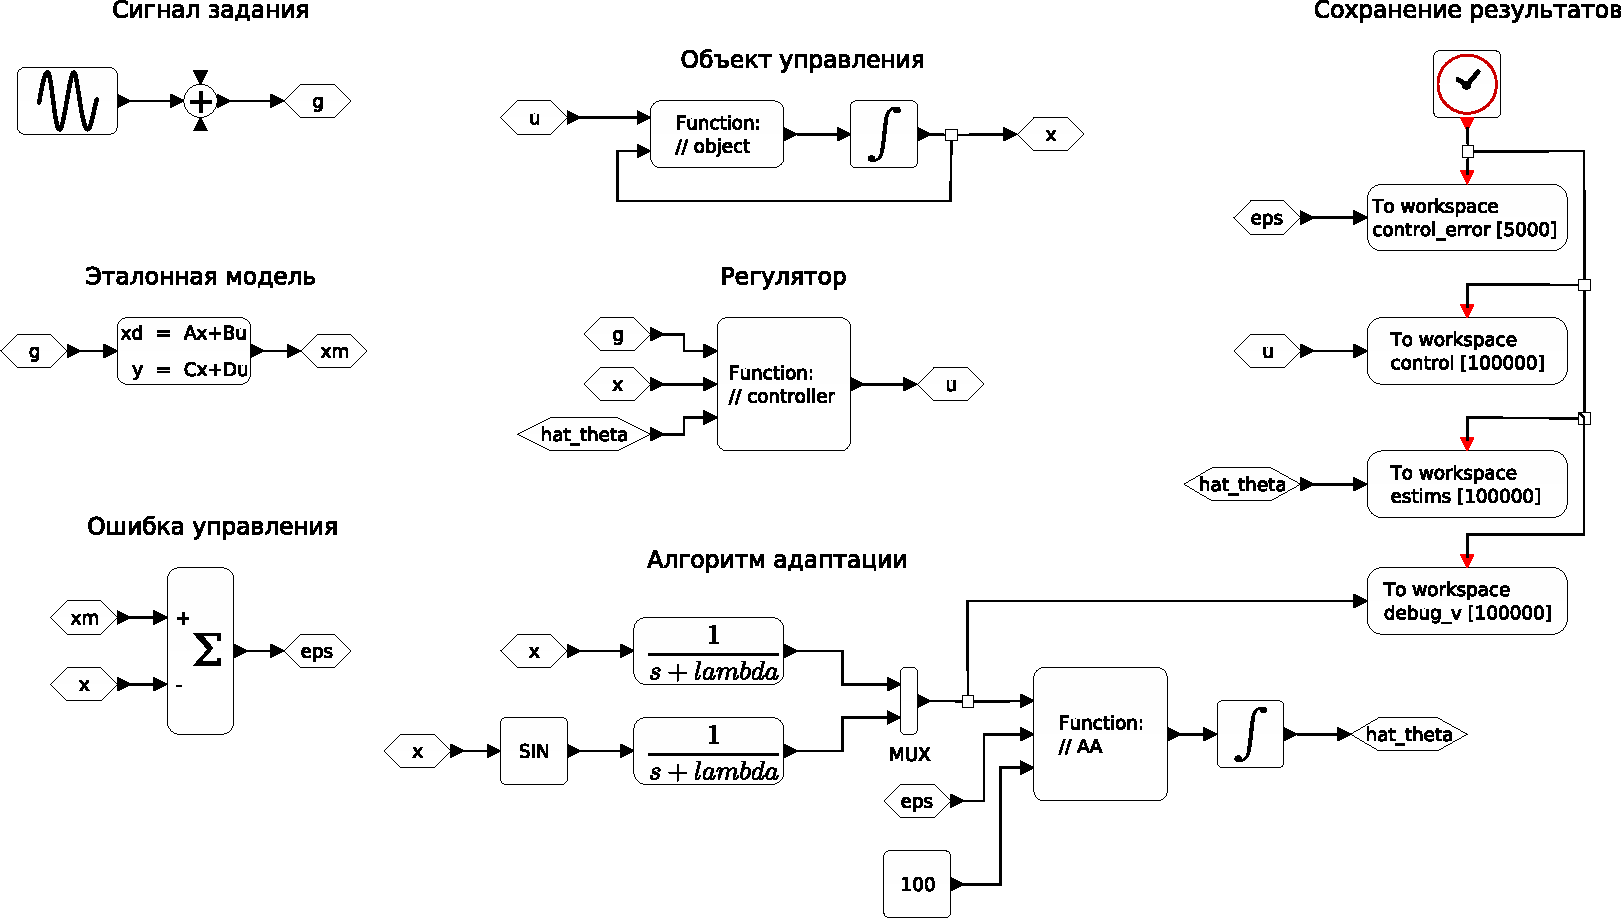
\includegraphics[width=\textwidth]{modeling_scheme.pdf}
    \vspace{0.5cm}
    \caption{Схема моделирования рассматриваемой системы.}
    \label{img_modeling_scheme}
\end{figure}


\section{Выводы по работе}
В~результате проделанной работы для заданного ОУ был рассчитан фильтр Калмана, оптимальным образом решающий проблему получения оценки его вектора состояния с точки зрения минимизации критерия~\eqref{eq_perfomance_index}.
Дополнительными экспериментами было установлено следующее:
\begin{itemize}
    \item при любых изменениях матрицы~$L$ относительно ее оптимального значения критерий качества получающегося при этом наблюдателя при $t \rightarrow \infty$ оказывается имеющим значения б\'oльшие, чем те, которые соответствуют~$J(t)$, характеризующему работу фильтра Калмана;
    \item при изменении спектральной плотности мощности шумов, действующих на систему, наблюдается следующая тенденция: при уменьшении первой~$J(t)$ уменьшается, а при увеличении~--- также увеличивается.
\end{itemize}
